
\subsection{Hypernym Discovery}

In order to organize all the primitive concepts into a fine-grained taxonomy,
we propose an active learning framework to iteratively 
discover isA relation between different primitive concepts.
To demonstrate the superior of our framework, 
we perform several experiments on a ground truth dataset collected after the taxonomy is constructed.
We randomly sample 3,000 primitive concepts in the class of ``\textit{Category}'' which have at least one hypernym, and retrieve 7,060 hyponym-hypernym pairs as positive samples.
We split the positive samples into training / validation / testing sets (7:2:1).
The search space of hypernym discovery is actually the whole vocabulary, 
making the number and quality of negative samples very important in this task.
The negative samples of training and validation sets are automatically generated from positive pairs
by replacing the hypernym of each pair with a random primitive concept from ``\textit{Category}'' class.
In the following experiments, mean average precision (MAP), mean reciprocal rank (MRR) and precision at rank 1 (P@1) are used as evaluation metrics. 

To verify the appropriate number of negative samples for each hyponym during training,
we perform an experiment shown in \figref{fig:isa}(left), 
where $N$ in x-axis represents the ratio of negative samples over positive samples for each hyponym.
The results indicate different size of negative samples influence the performance differently.
As $N$ gradually increases, the performance improves and achieves best around $100$.
Thus, we construct the candidate training pool in the following active learning experiment with a size of $500,000$.

\begin{figure}[th]
	\centering
	\epsfig{file=figures/isa.eps, width=\columnwidth}
	\caption{Left: the influence of different negative sample sizes in hypernym discovery on test set. Right: the best performance of different sampling strategies in active learning.}
	\label{fig:isa}
\end{figure}

\tabref{tab:isa} shows experimental results of different sampling strategies during our active learning framework, 
where $Random$ means training using the whole candidate pool without active learning.
We set the select data size $K$ as $25,000$ in each iteration as mentioned in \secref{sec:isa}.
When it achieves similar MAP score in four active learning strategies,
we can find that all the active learning sampling strategies can reduce labeled data to save considerable manual efforts.
UCS is the most economical sampling strategy, which only needs $325k$ samples, reducing $35\%$ samples comparing to random strategy.
It indicates that high confident negative samples are also important in the task of hypernym discovery.

\begin{table}[th]
	\centering
	%\scriptsize
	\begin{tabular}{l|c|c|c|c|c}
		\hline
		Strategy & Labeled Size &  MRR & MAP & P@1 & Reduce \\
		\hline
		Random & 500k & 58.97 & 45.30 & 45.50 & - \\
		US  & 375k &  59.66 & 45.73 & 46.00 & 150k\\
		CS & 400k &  58.96 & 45.22 & 45.30 & 100k\\
		UCS  & 325k &  59.87 & 46.32 & 46.00 & 175k \\
		\hline
	\end{tabular}
	\caption{Experimental results of different sampling strategy in hypernym discovery.}
	\label{tab:isa}
\end{table}

In \figref{fig:isa} (right), 
we show the best performance of each sampling strategies during the whole training procedure.
UCS outperforms other three strategies and achieves a highest MAP of $48.82\%$, showing the importance of selecting the most valuable samples during model training.




